\documentclass[10pt,a4paper]{article}
\usepackage[utf8x]{inputenc}
\usepackage{ucs}
\usepackage[english]{babel}
\usepackage{amsmath}
\usepackage{amsfonts}
\usepackage{amssymb}
\usepackage{makeidx}
\usepackage{graphicx}
\usepackage{lmodern}
\usepackage{kpfonts}
\usepackage{float}

\usepackage[left=2cm,right=2cm,top=2cm,bottom=2cm]{geometry}

\usepackage{titlesec}

\renewcommand{\o}{\circ}


% elimina newline despues de \section:
\titleformat{\section}[runin]
{\normalfont\large\bfseries}{\thesubsection}{1em}{}      


\headsep17mm
\topmargin-1cm
\hoffset -1.5cm \voffset -1cm \textwidth 17cm \oddsidemargin
1.5cm \evensidemargin 1.5cm \textheight 22.5cm

\begin{document}

\vspace{0,3cm}

\begin{center}
{\bf \Large Resoluciones seleccionadas, semana 02}
\end{center}

\vspace{0,3cm}

\section*{2.3.b}


\noindent
Para:

$ f(x) = 2x + 1$, \hspace{2cm} $g(x) = x^{3} - x^{2} - 4 $

\noindent
Calculamos $f \o g$, $g \o f$, $g + f$.


\noindent
\emph{Solución:}

\begin{align*}
  (f \o g)(x)
  &= f(g (x)) &\\
  &= 2g(x)+1 &\\
  &= 2 (x^3-x^2-4)+1 &\\
  &= 2x^3-2x^2-7 &\\ \\
  (g \o f)(x)
  &= g (f (x)) &\\
  &= g(x)^3-g(x)^2-4 &\\
  &= (2x+1)^3-(2x+1)^2-4 &\\
  &= 8 x^3 + 12 x^2 + 6 x + 1 - (4 x^2 + 4 x + 1) - 4 &\\
  &= (2x+1)^3-(2x+1)^2-4 & \\ \\
  (f + g) (x)
  &= f(x) + g (x) &\\
  &= 2x + 1 + x^3 - x^2 - 4 &\\
  &= x^3 - x^2 + 2x -3&
\end{align*}




\section*{2.3.i}


\noindent
Para

$$f(x) = \left \{ \begin{matrix} 0 & x \leq 0
\\ \frac{x}{2} & 0 < x < 4 
\\ 1- x & x \geq 4 \end{matrix}\right. , \hspace{1cm}
g(x) = \left \{ \begin{matrix} x +3 & x \leq 0
\\  \frac{1}{x} & x > 0 \end{matrix}\right.$$

Calculamos $f + g$ y $f \o g$.


\noindent
\emph{Solución:}

\noindent
$f + g$ como $f$ y $g$ están definidas en segmentos,
$f+g$ estará definida en segmentos, combinando las particiones.


\noindent
Tenemos que definir entonces $f+g$ en $(-\infty,0]$, $(0,4)$,
  y $[4,+\infty)$


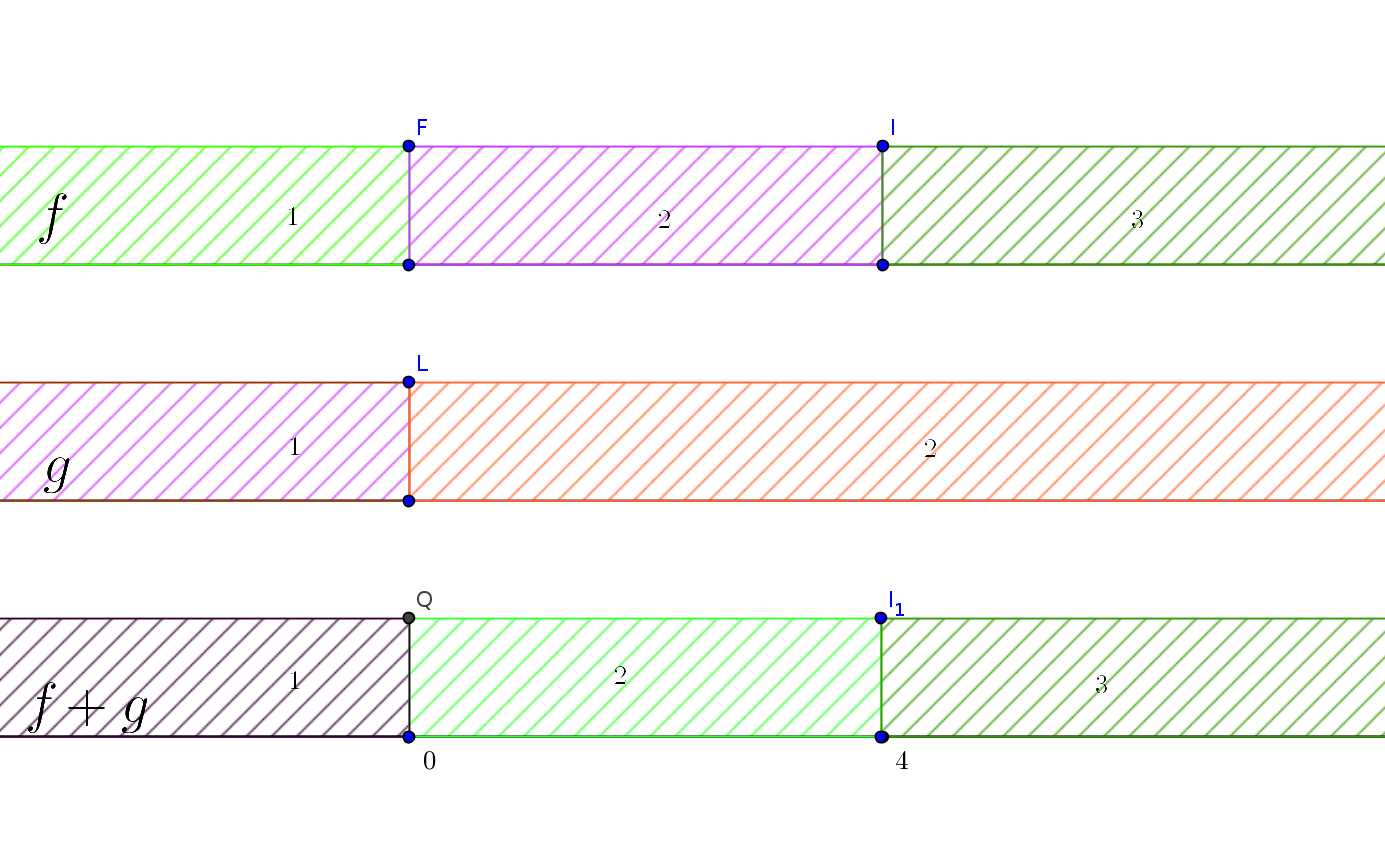
\includegraphics{suma.png}

\begin{enumerate}
\item Para $x \in (-\infty,0]$ tenemos que $f$ y $g$ se computan
  a partir de las expresiones $f(x) = 0$ y $g(x) = x + 3$.
  Luego $(f+g) (x) = 0 + x + 3$.

\item Para $x \in (0,4)$, $f(x) = \frac{x}{2}$ y $g(x) = \frac{1}{x}$.
  Luego $(f+g) (x) = \frac{x}{2} + \frac{1}{x} = \frac{x^2+2}{2x}$.

\item Para $x \in [4,\infty)$,  $f(x) = 1-x$ y $g(x) =  \frac{1}{x}$.
  Luego $(f+g) (x) = 1 - x + \frac{1}{x} = \frac{-x^2 + x + 1}{x}$
  
\end{enumerate}


Finalmente
$$(f+g)(x) = \left \{ \begin{matrix} x+3 & x \leq 0
\\ \frac{x^2+2}{2x} & 0 < x < 4 
\\ \frac{-x^2 + x + 1}{x} & x \geq 4 \end{matrix}\right. , \hspace{1cm}
\square $$
\newline
\noindent
Por otra parte, para hallar la composición aplicamos
$g$ y luego $f$ al resultado ($(f \o g)(x) = f (g (x)) $).

\noindent
Notemos que
$$f(g(x)) = \left \{ \begin{matrix} 0 & g(x) \leq 0
\\ \frac{g(x)}{2} & 0 < g(x) < 4 
\\ 1- g(x) & g(x) \geq 4 \end{matrix}\right. , \hspace{1cm}
$$



Estudiamos entonces para $g$ a qué intervalos pertenece la imagen,
según los casos de la definición:

\begin{enumerate}
\item
  \begin{itemize}
  \item
    Si $x \leq 0$ entonces $g(x) = x+3$. A continuación estudiamos cuando
  $x+3 \leq 0$, cuando $0 < x+3 < 4$ y cuando $x+3 \geq 4$ para ver qué
  expresión algebraica usar para $f(g(x))$.
  La forma sistemática de hacer esto es estudiar las soluciones de estas
  inecuaciones (el caso $0 < x+3 < 4$ es en realidad un sistema de dos
  inecuaciones).
  Tenemos que $x+3 \leq 0$ sii $x \leq -3$.
  Observemos que ésta solución hallada tiene
  sentido en el intervalo que estamos estudiando\footnote{esto es de alguna
  forma análogo a la resolución del ejercicio seleccionado del
  práctico anterior} ($(-\infty, 0]$),
  y en este caso como la solución está incluida en el mismo no se agrega
  ninguna nueva restricción.
  Para estos valores de $x$ entonces aplicamos la definición de $f$,
  y tenemos entonces que $f(g(x)) = 0$.
  \item Por otro lado es sencillo ver que si
  $x> -3$ (y además sabemos que $x<0$),
  $x+3$ cumple que $0<x-3<4$ y por tanto
  si $ -3 < x \leq 0$ luego $f(g(x)) = \frac{x+3}{2}$.
  \end{itemize}
\item Si $x > 0$ entonces $g(x) = \frac{1}{x}$.
  \begin{itemize}
  \item La inecuación $\frac{1}{x} \leq 0$ no tiene soluciones positivas,
    no vamos a elegir nunca aplicar $f$ según este segmento.

  \item La condición $0 < \frac{1}{x}< 4$ se cumple si $ x > \frac{1}{4}$.
    Para estos valores de $x$ entonces $(g\o f) (x) = \frac{1}{2x}$.
    
  \item Finalmente $\frac{1}{x} \geq 4$ se satisface cuando
    $x \leq \frac{1}{4}$, por tanto  $(g\o f) (x) = 1 - \frac{1}{x}$ en
    $(0,\frac{1}{4}]$
   
  \end{itemize}
  
\end{enumerate}


Entonces $g \o f$ queda definifa como:

$$
f(x) = \left \{
\begin{matrix} 0 & x \leq -3
  \\ \frac{x+3}{2} & -3 < x \leq 0 
  \\ 1- \frac{1}{x} &  0 < x \leq \frac{1}{4}
  \\ \frac{1}{2x} & x > \frac{1}{4}
\end{matrix}\right.
$$




\end{document}
